\documentclass{beamer}

\usepackage[english]{babel}
\usepackage[utf8]{inputenc}
\usepackage{graphicx}
\usepackage{booktabs}
\usepackage{hyperref}
\usepackage{tikz}
\usepackage{pgfplots}
\usepackage{amsmath, amssymb}
\usepackage{ragged2e}
\usepackage[T1]{fontenc}
\DeclareUnicodeCharacter{02BC}{'} % Define o caractere U+02BC como apóstrofo

\pgfplotsset{compat=1.16}
\usetikzlibrary{arrows.meta, positioning, shapes.geometric, patterns, decorations.pathreplacing, calc}

\mode<presentation>{\usetheme{default}\usecolortheme{default}\usefonttheme{default}}
\setbeamertemplate{caption}[numbered]
\setbeamertemplate{navigation symbols}{}

% --- Custom blocks ---
% Alert blocks (RED) → problems, limitations, warnings
\setbeamercolor{block title alerted}{bg=red!70!black, fg=white}
\setbeamercolor{block body alerted}{bg=red!10, fg=black}

% Example blocks (BLUE) → definitions, models
\setbeamercolor{block title example}{bg=blue!70!black, fg=white}
\setbeamercolor{block body example}{bg=blue!10, fg=black}

% Standard blocks (GRAY) → neutral content
\setbeamercolor{block title}{bg=gray!70, fg=white}
\setbeamercolor{block body}{bg=gray!10, fg=black}

% --- Placeholder for numbers still to be filled in ---
\newcommand{\todo}[1]{\textcolor{red}{\textbf{[#1]}}}

% --- Footer ---
\setbeamertemplate{footline}
{
  \leavevmode%
  \hbox{%
    \begin{beamercolorbox}[wd=.8\paperwidth,ht=2.5ex,dp=1.125ex,left]{author in head/foot}%
      \hspace{0.3cm}\insertshortauthor%
      \hspace{0.4cm}--\hspace{0.4cm}%
      \insertsection
    \end{beamercolorbox}%
    \begin{beamercolorbox}[wd=.2\paperwidth,ht=2.5ex,dp=1.125ex,right]{date in head/foot}%
      \insertframenumber{} / \inserttotalframenumber\hspace{0.3cm}
    \end{beamercolorbox}%
  }%
  \vskip0pt%
}

% --- Title ---
\title{\textbf{When to Repair? Emulator-Based Maintenance Optimization of Reinforced Concrete Under Carbonation}}
    % TODO: add co-authors (e.g., Victor Hugo, Renata, Maria)
    \author[W. M. Pereira Jr.]{\textbf{Prof. Wanderlei Malaquias Pereira Junior}}
    \institute{Federal University of Catalão \\ University of Minnesota}
\date{\today}


\begin{document}

% --- Slides ---
\begin{frame}[plain]
    \titlepage
\end{frame}

\begin{frame}{Agenda}
    \tableofcontents
\end{frame}
\section{About Me}
    \begin{frame}{About Me}

\begin{itemize}
    \item Civil Engineer
    \item MSc in Structural Engineering
    \item PhD in Science and Technology
    \item Assistant Professor at the Federal University of Catalão (Brazil)
    \item Research funded by the Brazilian National Council for Scientific and Technological Development (CNPq)
    \item Host institution: University of Minnesota (USA)
\end{itemize}

\end{frame}

\section{The maintenance problem}
    \begin{frame}{The Maintenance Problem}

\justifying

Owners of aging reinforced concrete structures must decide
\textbf{when to inspect} and \textbf{when to repair}, long before visible damage appears.

\vspace{0.4cm}

\begin{columns}[T,onlytextwidth]
  \column{0.48\textwidth}
  \begin{alertblock}{Repair too early}
  \justifying
  We pay for repairs the structure did not need yet.
  \end{alertblock}

  \column{0.48\textwidth}
  \begin{alertblock}{Repair too late}
  \justifying
  The steel is already corroding: the repair is more expensive and the risk is higher.
  \end{alertblock}
\end{columns}

\vspace{0.5cm}

\begin{block}{Research question}
\justifying
How often should we inspect, and at what condition should we repair, to minimize the life-cycle cost of a concrete element exposed to carbonation?
\end{block}

\end{frame}

    \begin{frame}{Carbonation and the Safety Margin}

\begin{columns}[c,onlytextwidth]

\column{0.42\textwidth}
\centering
\resizebox{\linewidth}{!}{%
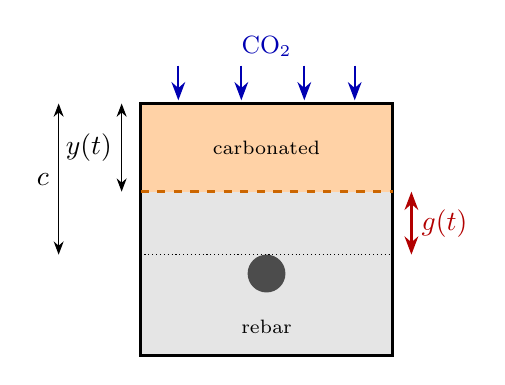
\begin{tikzpicture}[scale=0.8]
  \fill[gray!20] (0,0) rectangle (4,4);
  \fill[orange!35] (0,2.6) rectangle (4,4);
  \draw[thick] (0,0) rectangle (4,4);
  \foreach \x in {0.6,1.6,2.6,3.4}
    \draw[-{Stealth},thick,blue!70!black] (\x,4.6) -- (\x,4.05);
  \node[blue!70!black] at (2,4.9) {\small CO$_2$};
  \draw[very thick,orange!80!black,dashed] (0,2.6) -- (4,2.6);
  \fill[black!70] (2,1.3) circle (0.3);
  \draw[densely dotted] (0,1.6) -- (4,1.6);
  \draw[{Stealth}-{Stealth}] (-0.3,4) -- node[left] {$y(t)$} (-0.3,2.6);
  \draw[{Stealth}-{Stealth}] (-1.3,4) -- node[left] {$c$} (-1.3,1.6);
  \draw[{Stealth}-{Stealth},red!70!black,thick] (4.3,2.6) -- node[right] {$g(t)$} (4.3,1.6);
  \node at (2,0.45) {\scriptsize rebar};
  \node at (2,3.3) {\scriptsize carbonated};
\end{tikzpicture}%
}

\column{0.54\textwidth}
\justifying
CO$_2$ penetrates the concrete and lowers its pH. When the carbonation front reaches the rebar, the steel loses its protection (\emph{depassivation}).

\vspace{0.3cm}

\begin{exampleblock}{Safety margin = distance to the rebar}
\[
  g(t) = c - y(t)
\]
$c$: cover \quad $y(t)$: carbonation depth\\[2pt]
Depassivation: \; $g(t) \le 0$
\end{exampleblock}

\vspace{0.2cm}

{\small $g$ can be measured in the field (mm).}

\end{columns}

\end{frame}

    \begin{frame}{The Margin Is Uncertain}

\begin{columns}[c,onlytextwidth]

\column{0.52\textwidth}
\centering
\resizebox{\linewidth}{!}{%
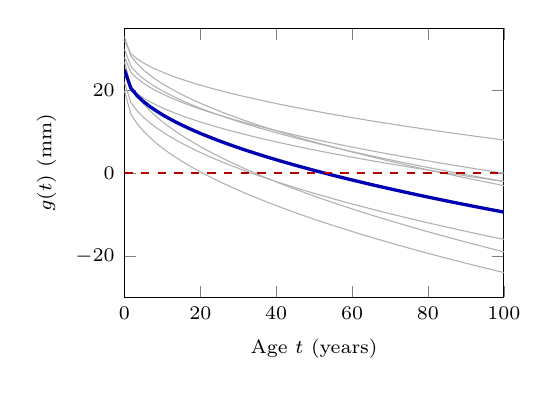
\begin{tikzpicture}
\begin{axis}[
  width=6.4cm, height=5.0cm,
  xlabel={Age $t$ (years)}, ylabel={$g(t)$ (mm)},
  xmin=0, xmax=100, ymin=-30, ymax=35,
  label style={font=\scriptsize}, tick label style={font=\scriptsize},
]
  \addplot[domain=0:100, samples=60, gray!60, thin] {32 - 2.4*sqrt(x)};
  \addplot[domain=0:100, samples=60, gray!60, thin] {28 - 2.8*sqrt(x)};
  \addplot[domain=0:100, samples=60, gray!60, thin] {22 - 3.8*sqrt(x)};
  \addplot[domain=0:100, samples=60, gray!60, thin] {30 - 3.2*sqrt(x)};
  \addplot[domain=0:100, samples=60, gray!60, thin] {20 - 4.4*sqrt(x)};
  \addplot[domain=0:100, samples=60, gray!60, thin] {27 - 4.6*sqrt(x)};
  \addplot[domain=0:100, samples=60, gray!60, thin] {24 - 2.6*sqrt(x)};
  \addplot[domain=0:100, samples=60, gray!60, thin] {33 - 3.6*sqrt(x)};
  \addplot[domain=0:100, samples=60, blue!70!black, very thick] {25 - 3.44*sqrt(x)};
  \addplot[red!70!black, thick, dashed] coordinates {(0,0) (100,0)};
\end{axis}
\end{tikzpicture}%
}

{\scriptsize Illustrative trajectories.}

\column{0.44\textwidth}
\justifying
Concrete strength, humidity, cover and CO$_2$ are uncertain, so each element follows a different trajectory.

\vspace{0.3cm}

\begin{exampleblock}{Probability of depassivation}
\[
  P_f(t) = P\left[g(t) \le 0\right]
\]
\end{exampleblock}

\vspace{0.2cm}

{\small Example (25 MPa, 25 mm cover): without maintenance, $P_f(100) \approx 0.88$.}

\end{columns}

\end{frame}

\section{Emulator}
    \begin{frame}{What Is an Emulator?}

\justifying

\begin{exampleblock}{Emulator}
\justifying
A fast statistical model trained on runs of a simulator. It replaces the simulator whenever we need to call it many times \cite{sacks_design_1989,kennedy_bayesian_2001}.
\end{exampleblock}

\vspace{0.3cm}

\centering
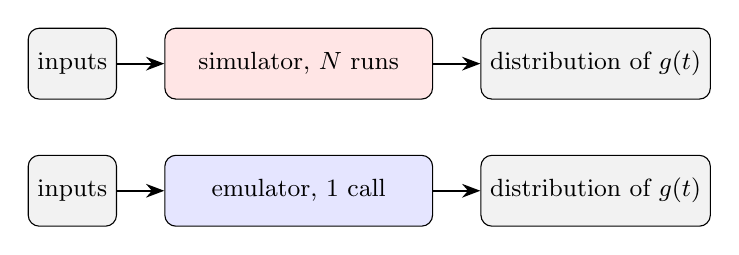
\begin{tikzpicture}[
  box/.style={draw, rounded corners, minimum height=0.9cm, align=center, font=\small},
  arr/.style={-{Stealth}, thick}
]
  \node[box, fill=gray!10] (in1) {inputs};
  \node[box, fill=red!10, right=0.6cm of in1, minimum width=3.4cm] (sim) {simulator, $N$ runs};
  \node[box, fill=gray!10, right=0.6cm of sim] (out1) {distribution of $g(t)$};
  \draw[arr] (in1) -- (sim);
  \draw[arr] (sim) -- (out1);

  \node[box, fill=gray!10, below=0.7cm of in1] (in2) {inputs};
  \node[box, fill=blue!10, right=0.6cm of in2, minimum width=3.4cm] (emu) {emulator, 1 call};
  \node[box, fill=gray!10, right=0.6cm of emu] (out2) {distribution of $g(t)$};
  \draw[arr] (in2) -- (emu);
  \draw[arr] (emu) -- (out2);
\end{tikzpicture}

\vspace{0.3cm}

\raggedright
Our emulator (neural network + Generalized Lambda Distribution) returns the \textbf{whole distribution} of $g(t)$ for a given design, at every age.

\end{frame}

    \begin{frame}{Why Use an Emulator Here?}

\justifying

Evaluating \emph{one} maintenance plan means simulating thousands of elements over 100 years, with repairs. The optimizer tests \emph{many} plans.

\vspace{0.3cm}

\begin{alertblock}{Without emulator}
\justifying
The physical model is called for every policy $\times$ every element $\times$ every repair cycle.
\end{alertblock}

\vspace{0.2cm}

\begin{exampleblock}{With emulator}
\justifying
The distribution of $g(t)$ is computed \textbf{once} per material (original concrete and repair mortar). All policies reuse it.
\end{exampleblock}

\vspace{0.3cm}

\raggedright
The same workflow applies to expensive models (finite elements, PDE solvers), where direct Monte Carlo is not feasible.

\end{frame}

\section{Optimization formulation}
    \begin{frame}{Maintenance Plan at the Design Stage}

\begin{columns}[c,onlytextwidth]

\column{0.56\textwidth}
\centering
\resizebox{\linewidth}{!}{%
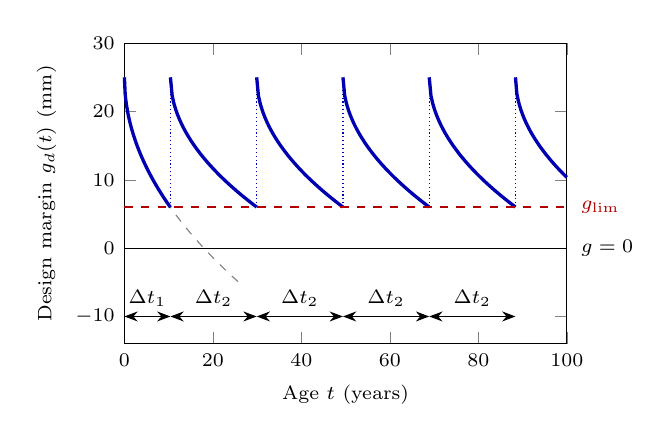
\begin{tikzpicture}
\begin{axis}[
  width=7.2cm, height=5.4cm,
  xlabel={Age $t$ (years)}, ylabel={Design margin $g_{d}(t)$ (mm)},
  xmin=0, xmax=100, ymin=-14, ymax=30,
  xtick={0,20,40,60,80,100},
  label style={font=\scriptsize}, tick label style={font=\scriptsize},
  clip=false,
]
  % no maintenance (original concrete)
  \addplot[domain=0:27, samples=60, gray, dashed] {25 - 5.9*sqrt(x)};
  % cycle 1: original concrete (reaches g_lim = 6 mm at t = 10.4 years)
  \addplot[domain=0:10.4, samples=60, blue!70!black, very thick] {25 - 5.9*sqrt(x)};
  % cycles 2+: repair mortar (reaches g_lim after 19.5 years)
  \addplot[domain=10.4:29.9, samples=50, blue!70!black, very thick] {25 - 4.3*sqrt(max(x-10.4,0))};
  \addplot[domain=29.9:49.4, samples=50, blue!70!black, very thick] {25 - 4.3*sqrt(max(x-29.9,0))};
  \addplot[domain=49.4:68.9, samples=50, blue!70!black, very thick] {25 - 4.3*sqrt(max(x-49.4,0))};
  \addplot[domain=68.9:88.4, samples=50, blue!70!black, very thick] {25 - 4.3*sqrt(max(x-68.9,0))};
  \addplot[domain=88.4:100, samples=40, blue!70!black, very thick] {25 - 4.3*sqrt(max(x-88.4,0))};
  % repairs
  \addplot[blue!70!black, densely dotted] coordinates {(10.4,6) (10.4,25)};
  \addplot[blue!70!black, densely dotted] coordinates {(29.9,6) (29.9,25)};
  \addplot[blue!70!black, densely dotted] coordinates {(49.4,6) (49.4,25)};
  \addplot[blue!70!black, densely dotted] coordinates {(68.9,6) (68.9,25)};
  \addplot[blue!70!black, densely dotted] coordinates {(88.4,6) (88.4,25)};
  % threshold and limit state
  \addplot[red!70!black, thick, dashed] coordinates {(0,6) (100,6)};
  \addplot[black, thin] coordinates {(0,0) (100,0)};
  \node[font=\scriptsize, red!70!black, anchor=west] at (axis cs:101,6) {$g_\mathrm{lim}$};
  \node[font=\scriptsize, anchor=west] at (axis cs:101,0) {$g = 0$};
  % intervals
  \draw[{Stealth}-{Stealth}] (axis cs:0,-10) -- node[above, font=\scriptsize] {$\Delta t_1$} (axis cs:10.4,-10);
  \draw[{Stealth}-{Stealth}] (axis cs:10.4,-10) -- node[above, font=\scriptsize] {$\Delta t_2$} (axis cs:29.9,-10);
  \draw[{Stealth}-{Stealth}] (axis cs:29.9,-10) -- node[above, font=\scriptsize] {$\Delta t_2$} (axis cs:49.4,-10);
  \draw[{Stealth}-{Stealth}] (axis cs:49.4,-10) -- node[above, font=\scriptsize] {$\Delta t_2$} (axis cs:68.9,-10);
  \draw[{Stealth}-{Stealth}] (axis cs:68.9,-10) -- node[above, font=\scriptsize] {$\Delta t_2$} (axis cs:88.4,-10);
\end{axis}
\end{tikzpicture}%
}

{\scriptsize Illustrative: $c = 25$~mm, $g_\mathrm{lim} = 6$~mm. Gray dashed: no maintenance.}

\column{0.41\textwidth}
\raggedright
Design stage: nothing to inspect yet, but we \textbf{know the model}.

\vspace{0.2cm}

\textbf{Rule}\\
Repair when the design margin $g_d(t)$ reaches $g_\mathrm{lim}$.

\vspace{0.2cm}

\begin{exampleblock}{Design margin}
\raggedright
$g_d(t)$: 5\% quantile of the emulator cloud (characteristic value).
\end{exampleblock}

\vspace{0.1cm}

{\small $\Delta t_1$: original concrete.\\
$\Delta t_2$: repair mortar (different carbonation rate).}

\end{columns}

\end{frame}

    \begin{frame}{Decision Variable}

\justifying

\begin{exampleblock}{$g_\mathrm{lim}$: repair threshold (mm)}
\justifying
Distance from the carbonation front to the rebar that triggers a repair.
It defines the whole maintenance schedule $t_1, t_2, \dots$
\end{exampleblock}

\vspace{0.3cm}

\begin{columns}[T,onlytextwidth]
  \column{0.48\textwidth}
  \textbf{Large $g_\mathrm{lim}$}
  \begin{itemize}
    \item Repair early
    \item Many repairs
    \item Few failures
  \end{itemize}

  \column{0.48\textwidth}
  \textbf{Small $g_\mathrm{lim}$}
  \begin{itemize}
    \item Repair late
    \item Few repairs
    \item Many failures
  \end{itemize}
\end{columns}

\vspace{0.3cm}

\begin{block}{Why a threshold and not a fixed interval?}
\justifying
The original concrete and the repair mortar carbonate at different rates.
A threshold in mm gives a different interval for each cycle, and it is the language engineers use in the field.
\end{block}

\end{frame}

    \begin{frame}{Objective Function}

\justifying

\begin{exampleblock}{Expected life-cycle cost over $T = 100$ years}
\[
  C_T(g_\mathrm{lim}) = \underbrace{c_\mathrm{rep}\, N_\mathrm{rep}(g_\mathrm{lim})}_{\text{planned repairs}}
  + \underbrace{c_\mathrm{fail}\, \mathbb{E}\left[N_\mathrm{fail}(g_\mathrm{lim})\right]}_{\text{failures in service}}
\]
\end{exampleblock}

\vspace{0.2cm}

\begin{itemize}
  \item $N_\mathrm{rep}$: number of planned repairs (known once $g_\mathrm{lim}$ is fixed).
  \item $N_\mathrm{fail}$: times the \emph{real} margin reaches $g(t) = 0$ before the planned repair (random, from the emulator cloud).
  \item A failure in service triggers a corrective repair and the element restarts.
  \item Costs relative to $C_0$, the construction cost of the element.
\end{itemize}

\vspace{0.1cm}

\centering
\begin{tabular}{@{}llc@{}}
\toprule
\textbf{Cost} & \textbf{Meaning} & \textbf{Initial value} \\ \midrule
$c_\mathrm{rep}$ & planned (preventive) repair & $0.10\, C_0$ \\
$c_\mathrm{fail}$ & corrective repair + indirect costs & $0.50\, C_0$ \\ \bottomrule
\end{tabular}

\end{frame}

    \begin{frame}{Expected Trade-Off}

\begin{columns}[c,onlytextwidth]

\column{0.55\textwidth}
\centering
\resizebox{\linewidth}{!}{%
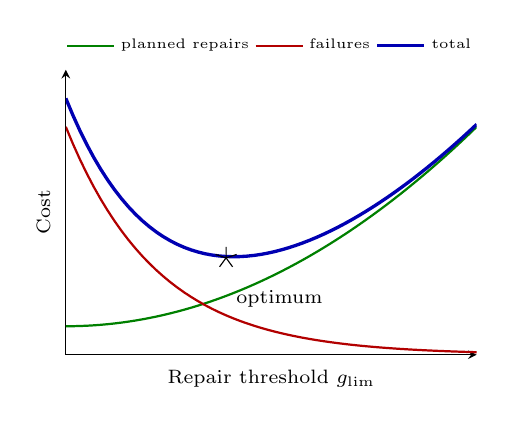
\begin{tikzpicture}
\begin{axis}[
  width=6.8cm, height=5.2cm,
  xlabel={Repair threshold $g_\mathrm{lim}$}, ylabel={Cost},
  xmin=0, xmax=10, ymin=0, ymax=10,
  xtick=\empty, ytick=\empty,
  axis lines=left,
  label style={font=\scriptsize},
  legend style={font=\tiny, at={(0.5,1.02)}, anchor=south, legend columns=3, draw=none},
]
  \addplot[domain=0:10, samples=60, green!50!black, thick] {1 + 0.07*x^2};
  \addplot[domain=0:10, samples=60, red!70!black, thick] {8*exp(-0.45*x)};
  \addplot[domain=0:10, samples=60, blue!70!black, very thick] {1 + 0.07*x^2 + 8*exp(-0.45*x)};
  \legend{planned repairs, failures, total}
  \addplot[only marks, mark=star, mark size=4pt, black] coordinates {(3.9,3.4)};
  \node[font=\scriptsize, anchor=north] at (axis cs:5.2,2.6) {optimum};
\end{axis}
\end{tikzpicture}%
}

{\scriptsize Qualitative sketch (no results yet).}

\column{0.42\textwidth}
\justifying
\begin{itemize}
  \item \textbf{Small $g_\mathrm{lim}$}: few planned repairs, many failures.
  \item \textbf{Large $g_\mathrm{lim}$}: few failures, many planned repairs.
  \item We expect an \textbf{interior optimum}.
  \item The optimum depends on the ratio $c_\mathrm{fail} / c_\mathrm{rep}$.
\end{itemize}

\end{columns}

\end{frame}

    \begin{frame}{Optimization Problem}

\justifying

\begin{exampleblock}{Formulation}
\[
\begin{aligned}
  \min_{g_\mathrm{lim}} \quad & c_\mathrm{rep}\, N_\mathrm{rep}(g_\mathrm{lim})
  + c_\mathrm{fail}\, \mathbb{E}\left[N_\mathrm{fail}(g_\mathrm{lim})\right] \\[6pt]
  \text{subject to} \quad & 0 \le g_\mathrm{lim} \le c_\mathrm{nom}
\end{aligned}
\]
\end{exampleblock}

\vspace{0.3cm}

\textbf{How each evaluation works}
\begin{enumerate}
  \item Build the schedule $t_1, t_2, \dots$ from the design margin $g_d(t)$ and $g_\mathrm{lim}$.
  \item Simulate many virtual elements from the emulator cloud over 100 years with this schedule.
  \item Count the failures in service and average them: $\mathbb{E}[N_\mathrm{fail}]$.
\end{enumerate}

\vspace{0.2cm}

{\small One variable: a simple scan over $g_\mathrm{lim}$ is enough to find the optimum.}

\end{frame}

    \begin{frame}{Planned Parametric Study}

\justifying

\textbf{Main study: how much does a failure cost?}

\vspace{0.15cm}

\centering
\begin{tabular}{@{}lccccc@{}}
\toprule
 & \textbf{low} & \textbf{base} & \multicolumn{2}{c}{\textbf{high}} & \textbf{extreme} \\ \midrule
$c_\mathrm{fail}$ & $0.3\, C_0$ & $0.5\, C_0$ & $1.0\, C_0$ & $2.0\, C_0$ & $20\, C_0$ \\
$c_\mathrm{fail} / c_\mathrm{rep}$ & 3 & 5 & 10 & 20 & 200 \\ \bottomrule
\end{tabular}

{\scriptsize $c_\mathrm{rep} = 0.10\, C_0$ fixed.}

\vspace{0.3cm}

\raggedright
\begin{columns}[T,onlytextwidth]
  \column{0.48\textwidth}
  \textbf{We will show}
  \begin{itemize}
    \item Total cost $C_T(g_\mathrm{lim})$, one curve per $c_\mathrm{fail}$
    \item Optimal $g^{\ast}_\mathrm{lim}$ vs. $c_\mathrm{fail}/c_\mathrm{rep}$
    \item At the optimum: $N_\mathrm{rep}$, $\mathbb{E}[N_\mathrm{fail}]$ and the repair schedule
  \end{itemize}

  \column{0.48\textwidth}
  \textbf{Secondary studies}
  \begin{itemize}
    \item Cover $c$: 20, 25, 30, 40 mm
    \item Concrete strength $f_c$: 25, 35, 50 MPa
    \item Humidity $RH$: 55\%, 75\%
    \item Design quantile of $g_d$: 5\%, 50\%
  \end{itemize}
\end{columns}

\vspace{0.2cm}

{\small Expected: the higher the failure cost, the larger $g^{\ast}_\mathrm{lim}$ and the more planned repairs.}

\end{frame}

    \begin{frame}{Open Questions and Next Steps}

\justifying

\textbf{Open questions}
\begin{enumerate}
  \item \textbf{Failure cost:} which range of $c_\mathrm{fail}/c_\mathrm{rep}$ is realistic for a serviceability failure?
  \item \textbf{Design margin:} which quantile of the cloud defines $g_d(t)$ (5\%, median)?
  \item \textbf{Discounting:} should future costs be discounted to present value?
  \item \textbf{End of horizon:} how to value the condition of the element at 100 years?
\end{enumerate}

\vspace{0.3cm}

\begin{block}{Next step: from design to operation}
\justifying
Once the structure is built, inspections measure the real margin and update the plan.
The design-stage plan becomes the starting point; inspections tell us when to deviate from it.
\end{block}

\end{frame}


% --- Old talk (kept for reference) ---
% \section{Research project}
%     \begin{frame}{Digital Models Philosophy}

% --- Definition (blue block) ---
\begin{block}{Digital Model}
\justifying
A Digital Model can be defined as a structured computational representation of a real physical system,
developed with the purpose of simulating, analyzing, and predicting the system’s behavior under different
operational conditions.
\end{block}

\vspace{0.3cm}

\textbf{My Goals}

\begin{columns}[T,onlytextwidth]
  \column{0.5\textwidth}
  \begin{itemize}
    \item Improve numerical simulations using real datasets
    \item Enhance numerical simulations through probabilistic theory
  \end{itemize}

  \column{0.5\textwidth}
  \begin{itemize}
    \item Prepare numerical models for digital twins
  \end{itemize}
\end{columns}

\end{frame}

% \section{Low-fidelity prototypes}
%     \begin{frame}{Cellular Automata for Chloride Ingress}

\justifying

\textbf{Research Question}

How can gas ingress into a concrete surface be simulated while probabilistically
quantifying the resulting material deterioration over time?

\vspace{0.20cm}

\textbf{How do researchers address this type of problem?}

Using fixed meso-scale representations for aggregate simulation.

\vspace{0.20cm}

\textbf{What are the limitations?}

This approach does not consider the effects of aggregate size variability
and spatial distribution within the cement matrix.

\end{frame}

%     \begin{frame}{Cellular Automata for Chloride Ingress}

\justifying

\textbf{How are we resolving this issue?}

By employing cellular automata coupled with the two-dimensional form of
Fick’s law and a probabilistic representation of aggregate dispersion.

\vspace{0.20cm}

\begin{block}{Cellular Automata} 
\justifying A cellular automaton is a discrete computational model composed of a lattice of cells, where each cell evolves in time according to local interaction rules based on the states of its neighboring cells. Cellular automata are particularly suitable for modeling spatially distributed physical processes. \end{block}

\vspace{0.20cm}

\textbf{Physical Background (Fick’s Law)}

\vspace{0.2cm}

\begin{equation}
\frac{\partial C(x,y,t)}{\partial t}
=
D
\left(
\frac{\partial^2 C(x,y,t)}{\partial x^2}
+
\frac{\partial^2 C(x,y,t)}{\partial y^2}
\right)
\label{eq:fick_2d}
\end{equation}

\end{frame}

%     \begin{frame}{Cellular Automata for Chloride Ingress}

\justifying

\textbf{Step 1: Aggregate Dataset Generation}

A DDPM is employed to generate a synthetic
aggregate dataset, capturing variability in size, shape, and spatial distribution
consistent with meso-scale representations of concrete.

\vspace{0.15cm}

\textbf{Step 2: Patch Construction}

The generated aggregates are assembled into spatial patches, which serve as the
computational domain for subsequent modeling of transport phenomena and material
deterioration.

\vspace{0.15cm}

\textbf{Step 3: Model Calibration}

The model is calibrated using the DE algorithm,
based on experimental chloride ingress data reported by \cite{DU201487}.

\vspace{0.15cm}

\textbf{Step 4: Numerical Simulation}

Simulations are performed on a concrete prism with dimensions
$75 \times 75$~mm to evaluate the chloride penetration front,
considering a concrete cover depth of 30~mm.

\end{frame}

%     \begin{frame}{Cellular Automata for Chloride Ingress}

\begin{figure}
\centering

\includegraphics[width=0.5\textwidth]{figures/concrete_mask.png}
\caption{Generated aggregate patches using DDPM.}
\label{fig:ddpm_patches}
\end{figure}

\end{frame}
%     \begin{frame}{Cellular Automata for Chloride Ingress}

\begin{figure}
\centering
\begin{columns}[T,onlytextwidth]

\column{0.48\textwidth}
\centering
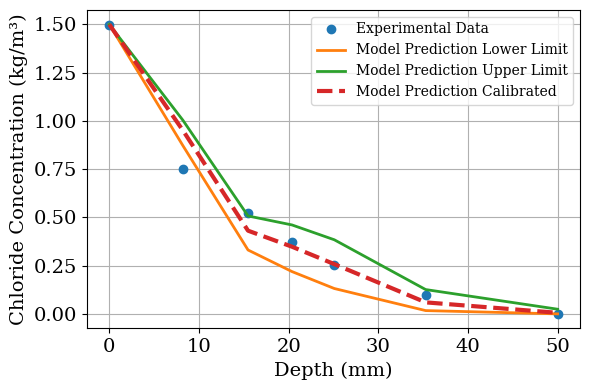
\includegraphics[width=\textwidth]{figures/calibration.png}\\
(a) Calibration with DE

\column{0.48\textwidth}
\centering
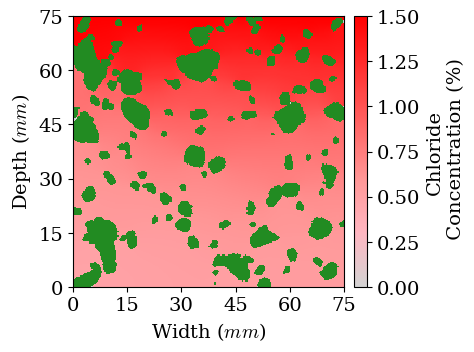
\includegraphics[width=\textwidth]{figures/simulation.png}\\
(b) First simulation

\end{columns}
\caption{Model calibration results and first simulation.}
\label{fig:model_calibration}
\end{figure}

\end{frame}
% \section{Improve analytical models}
%     \begin{frame}{Enrichment for crack models}

\justifying

\textbf{Research Question}

How can genetic programming be used to develop improved analytical models for crack width prediction?

\vspace{0.20cm}

\textbf{How do researchers address this type of problem?}

Using black box models (machine learning/artificial intelligence).

\vspace{0.20cm}

\textbf{What are the limitations?}

The forecasting mechanism is not transparent, and the AI model is required for all predictions \cite{zhang_explainable_2025}.

\end{frame}

%     \begin{frame}{Enrichment for Crack Models}

\justifying

\textbf{How are we resolving this issue?}

Employing Genetic Programming to predict the discrepancy between experimental data and analytical model predictions.

\vspace{0.15cm}

\begin{block}{Discrepancy modeling}
\justifying 
Model calibration finds optimal parameters $\boldsymbol{\theta}^{\ast}$ that minimize differences between observed data $\mathbf{d}$ and model predictions $\mathbf{q}(\boldsymbol{\theta})$. However, measurement noise $\varepsilon_i$ and model-form uncertainty (structural inadequacy) prevent perfect matching. Following \cite{brynjarsdottir_learning_2014}, we incorporate an explicit discrepancy term $\delta(\boldsymbol{\theta}, \epsilon_i)$ to account for missing physics or scale effects.
\end{block}

\vspace{0.20cm}

\textbf{Discrepancy equation}

\vspace{0.2cm}

\begin{equation}
    \label{eq:discrepancy_model}
    d_i = q_i(\boldsymbol{\theta}) + \delta(\boldsymbol{\theta}, \epsilon_i) + \varepsilon_i'
\end{equation}

\end{frame}
%     \begin{frame}{Enrichment for Crack Models}

\begin{figure}
\centering
\begin{columns}[T,onlytextwidth]

\column{0.48\textwidth}
\centering
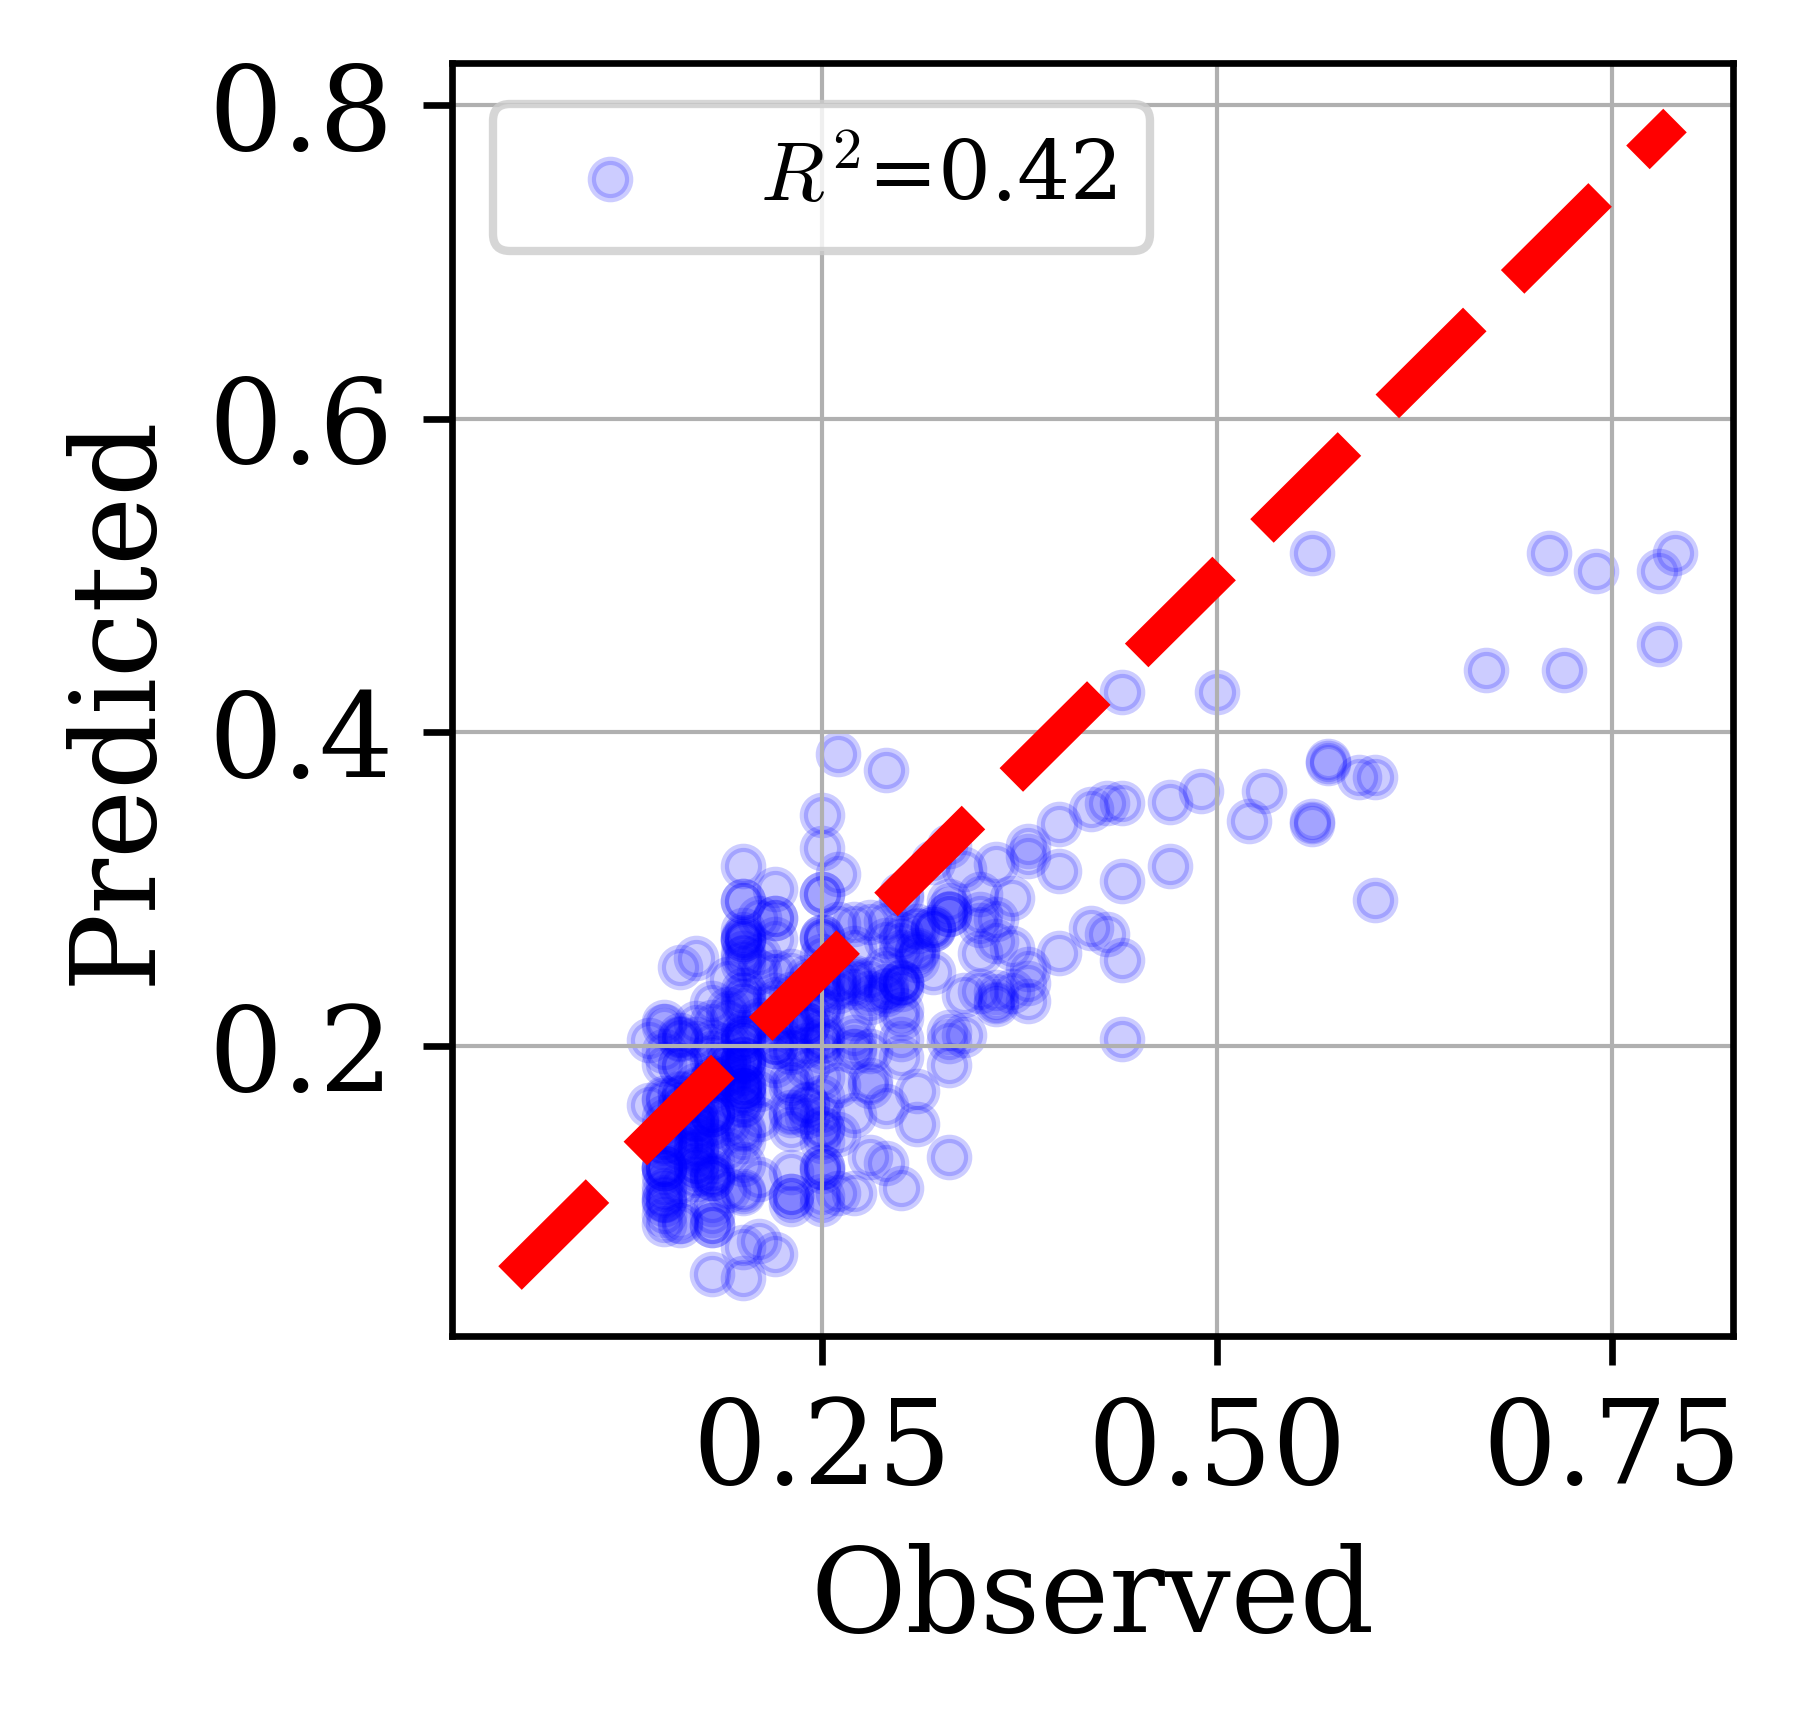
\includegraphics[width=\textwidth]{figures/z_scatter-line_fib_model_2020.png}\\
(a) fib Model Code 2020 (original)

\column{0.48\textwidth}
\centering
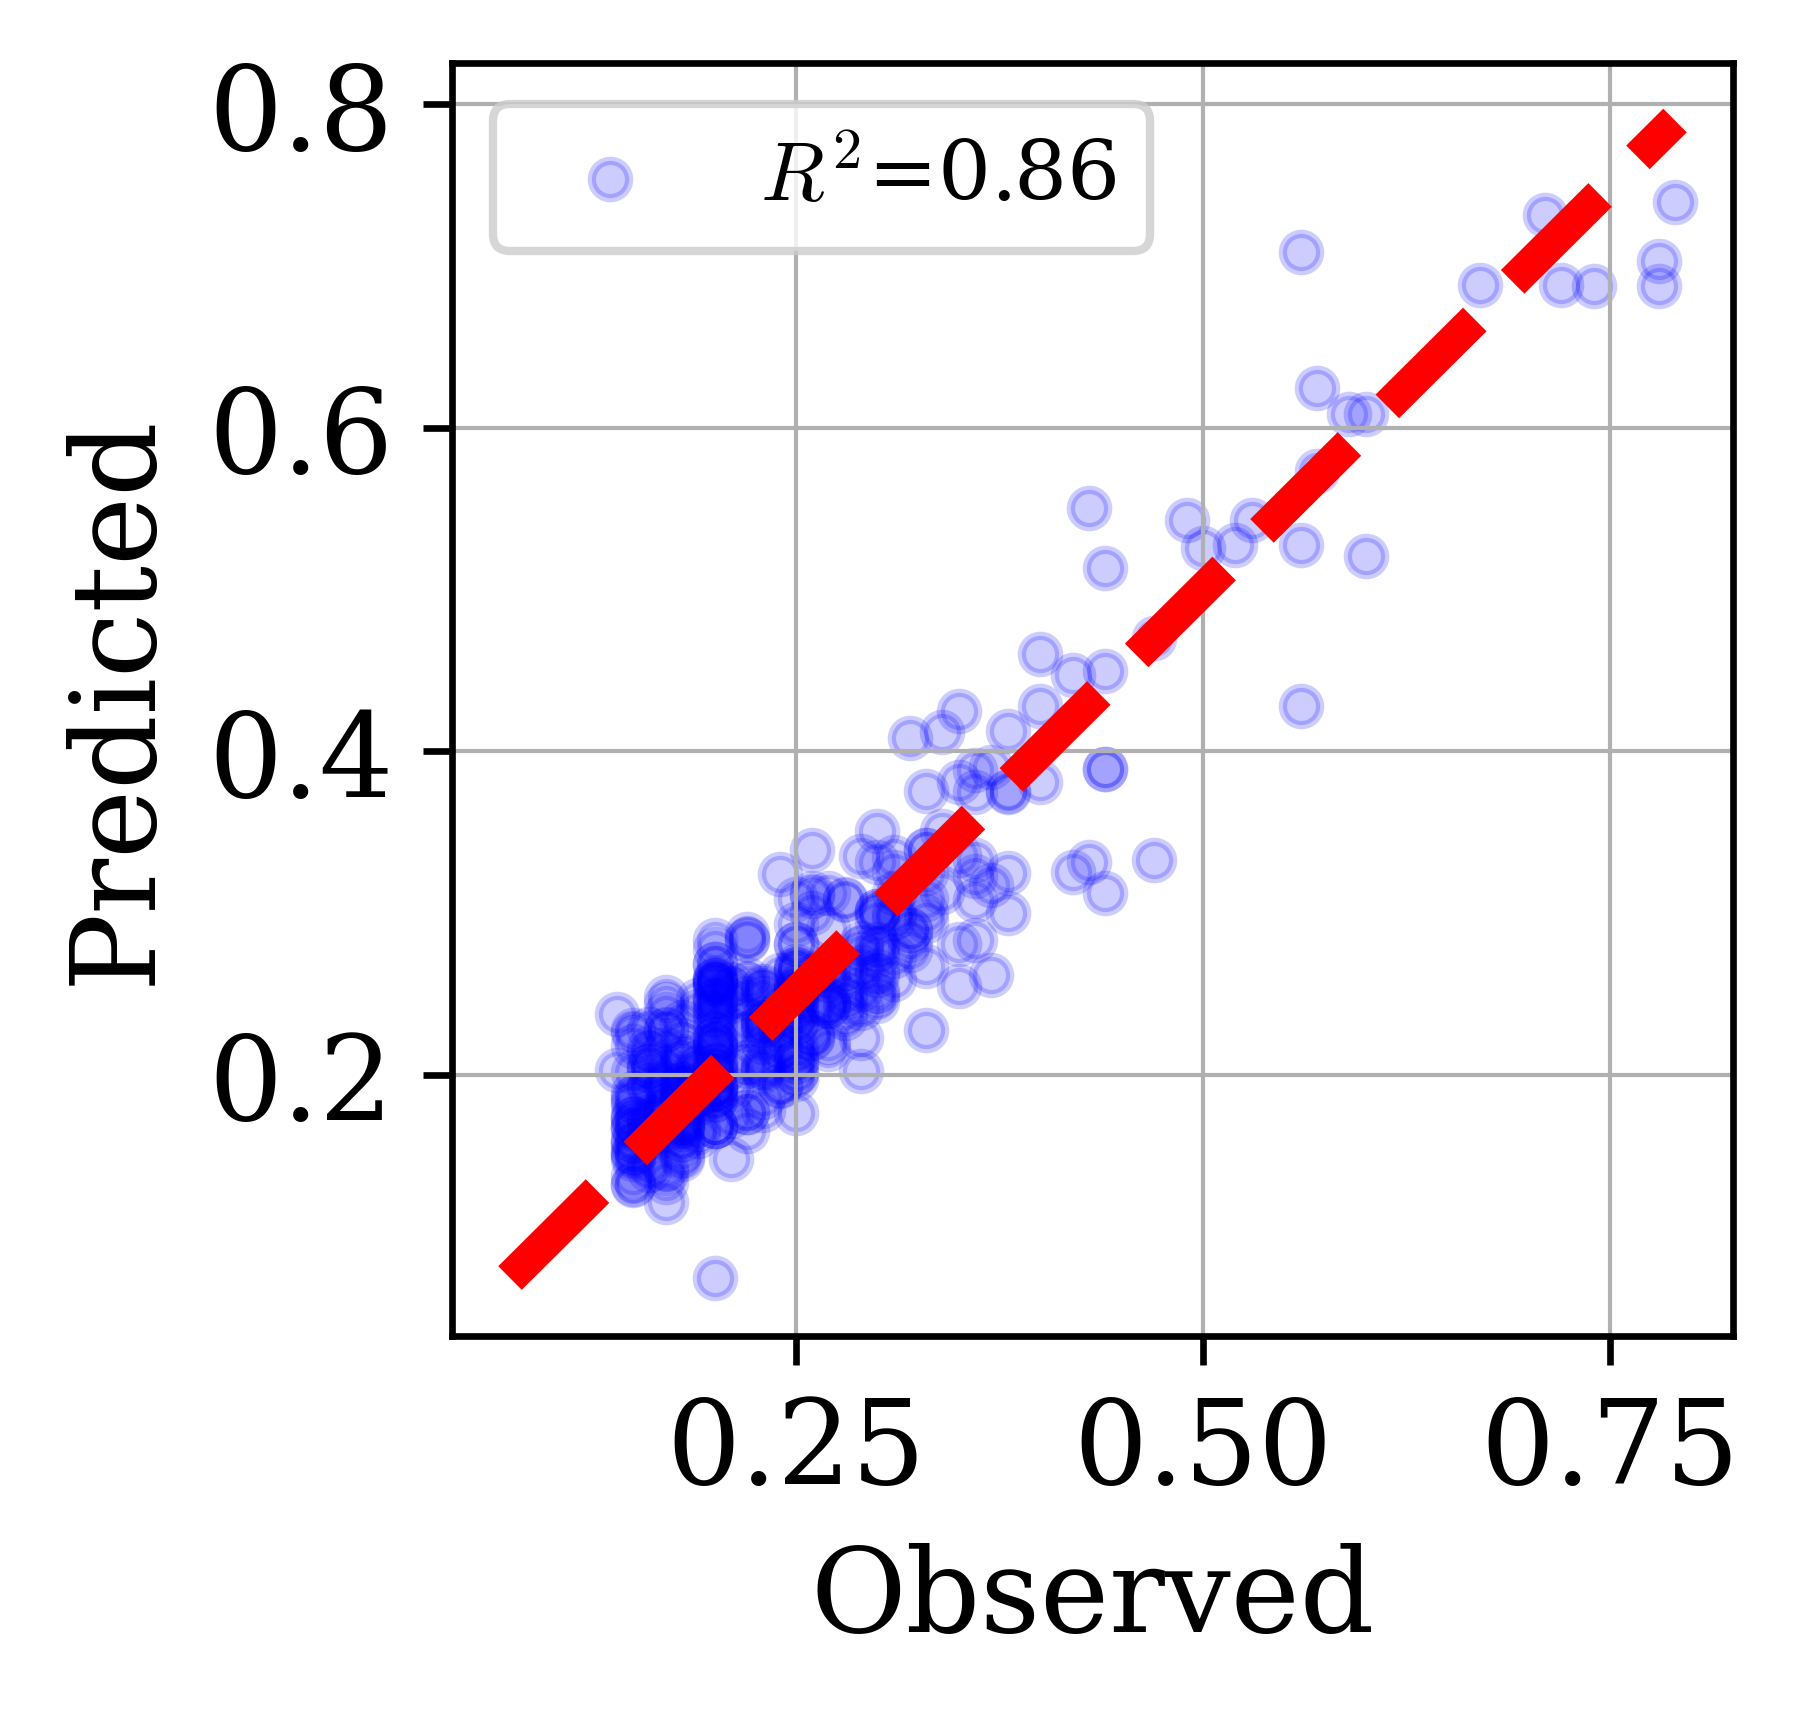
\includegraphics[width=\textwidth]{figures/z_scatter-line_fib_model_2020-pysr-model-dataset-1-8020.png}\\
(b) fib Model Code 2020 (enriched)

\end{columns}
\caption{Original vs. enriched crack prediction models.}
\label{fig:model_calibration}
\end{figure}

\end{frame}

\section{References}

\begin{frame}[allowframebreaks]{References}
\tiny
\bibliography{references}
\bibliographystyle{apalike}
\end{frame}

\begin{frame}[plain]

\vspace{1.2cm}

% {\Large\bfseries Obrigado}

% \vspace{0.3cm}

{\Large\bfseries Thank you}

% \vspace{0.3cm}

% {\Large\bfseries 谢谢}

% \vspace{1.0cm}

{\normalsize
Prof. Wanderlei Malaquias Pereira Junior
}

\vspace{0.5cm}

{\small
\texttt{wanderlei\_junior@ufcat.edu.br}\\
\texttt{wjunior@umn.edu}
}

\vfill

\end{frame}


\end{document}
